\documentclass[11pt]{article}

\usepackage[a4paper,margin=1in]{geometry}
\usepackage[T1]{fontenc}
\usepackage[utf8]{inputenc}
\usepackage{lmodern}
\usepackage{microtype}
\usepackage{graphicx}
\usepackage{booktabs}
\usepackage{array}
\usepackage{enumitem}
\usepackage{hyperref}
\usepackage{xcolor}
\usepackage{tikz}
\usetikzlibrary{arrows.meta,positioning,fit,shapes.geometric}

\hypersetup{
  colorlinks=true,
  linkcolor=blue!55!black,
  citecolor=blue!55!black,
  urlcolor=blue!55!black
}

\title{\textbf{MoonAP v0.1: A MoonBit Agent Playground for LLM-Generated Browser-Local WebAssembly Applications}}
\author{
  Maomao Tang\\
  CUHK-SZ\\
  \texttt{maomaotang@link.cuhk.edu.cn}
}
\date{April 2026}

\newcommand{\moonap}{MoonAP}
\newcommand{\skill}{SKILL}
\newcommand{\wasm}{WebAssembly}
\newcolumntype{L}[1]{>{\raggedright\arraybackslash}p{#1}}

\begin{document}
\maketitle

\begin{abstract}
Large language models (LLMs) can synthesize useful programs from natural-language descriptions, but source code alone is not yet a complete application experience. A practical software synthesis environment must compile generated code, provide inputs, execute safely, present results, preserve useful artifacts, and avoid unnecessary movement of private data. This paper presents \moonap{} v0.1, a MoonBit-oriented agent playground that turns a natural-language request into MoonBit source code, compiles it to \wasm{}, runs it locally in the browser, and saves successful applications as reusable \moonap{}-\skill{} packages. The system combines an LLM routing layer, a MoonBit compilation service, declarative runtime contracts, browser-local file execution, and a three-layer \skill{} architecture for personal reuse, local installation, and cloud discovery. The v0.1 prototype demonstrates twelve task categories, from calculators and JSON/text utilities to CSV analysis and large FastQ generation/analysis. Its main contribution is a platform pattern for LLM-generated applications where raw user files remain on the client, browser-side computation handles large inputs, and saved \skill{}s can be rerun without repeated LLM calls. We also report a pragmatic lesson from targeting a young language: when real lightweight models do not yet generate MoonBit reliably, deterministic simulation paths, explicit runtime contracts, and artifact reuse are essential for building and evaluating the surrounding synthesis system.
\end{abstract}

\section{Introduction}

LLM-based software synthesis has made it possible for users to describe a program in natural language and receive source code~\cite{chen2021evaluating,austin2021program,li2022competition}. Most benchmarks and demonstrations emphasize the generation step: whether the model can produce a correct function, solve a programming problem, or pass tests. In everyday use, however, generated source code is only one part of the path to a working application. A practical system must select or configure a model, preserve prompts and generated source, compile the program, expose runtime inputs, execute the artifact, present results, and allow successful programs to be reused. These requirements become more pronounced when the target language is new, when the generated program is intended to run in a browser, or when user data should remain local.

\moonap{} is a MoonBit Agent Playground designed to explore this complete workflow. A user describes an application, the system asks an LLM to generate MoonBit code, a local server compiles the code to \wasm{}, and the browser runs the resulting application with a task-specific runtime UI. If the result is useful, the application can be saved as a \moonap{}-\skill{} and reused later without another LLM call. In this model, the LLM is used to create or repair an application, while routine execution shifts to the user's machine.

MoonBit is a young programming language with a toolchain oriented toward modern application targets, including \wasm{}~\cite{moonbit,webassembly}. This makes it attractive for browser-local synthesized applications, but it also exposes a difficulty: many lightweight or free LLM routes do not yet generate valid MoonBit code consistently. \moonap{} therefore treats code generation as only one part of the system. It pairs real API routes with deterministic simulated routes, embeds runtime specifications in generated artifacts, and separates generation-time behavior from reuse-time behavior.

This paper reports on \moonap{} v0.1 as a system prototype. The contribution is a working architecture for connecting LLM-generated MoonBit code to browser-local execution and reuse:

\begin{itemize}[leftmargin=*]
  \item an end-to-end pipeline from natural-language task to MoonBit source, \wasm{} compilation, browser-local execution, and reusable \skill{};
  \item a runtime contract abstraction for generated applications, covering form, text, report, file, and large-file workflows;
  \item a three-layer \skill{} model that distinguishes personal reuse, locally installed public \skill{}s, and cloud discovery;
  \item browser-local large-file workflows for FastQ generation and analysis, including streamed and chunked processing paths designed for GB-scale files whose raw contents remain on the client;
  \item a data-local execution model in which raw files are processed near the user and successful applications can be rerun without repeated generation;
  \item an implementation and qualitative evaluation over twelve v0.1 demonstration categories.
\end{itemize}

\section{Related Work and Positioning}

\paragraph{LLM program synthesis.}
Prior work has shown that large language models can synthesize code from natural-language prompts and solve programming tasks at increasing levels of difficulty~\cite{chen2021evaluating,austin2021program,li2022competition}. \moonap{} builds on this line of work but studies a different part of the lifecycle. Instead of asking only whether a model can emit correct source code, \moonap{} asks how generated code becomes a runnable, inspectable, reusable, and locally executed application.

\paragraph{MoonBit and \wasm{}.}
MoonBit targets modern software delivery scenarios, and \wasm{} provides a portable execution target for browser and non-browser environments~\cite{moonbit,webassembly}. This combination is well suited to synthesized client-side tools: generated code can be compiled into an artifact that the browser can host, while the surrounding system controls UI, file access, and result presentation.

\paragraph{Browser-local file access.}
\moonap{} relies on browser file picker and file system capabilities for local workflows. The File System Access API is developed through the Web Platform Incubator Community Group, and browser compatibility remains narrower than baseline web APIs~\cite{file-system-access,mdn-file-system-access}. For this reason, v0.1 validates large-file workflows primarily in Chrome and Edge rather than claiming universal browser support.

\paragraph{Safety and artifact reuse.}
Generated code can introduce security and provenance risks, as prior studies of AI-assisted code generation have emphasized~\cite{pearce2022asleep}. \moonap{} v0.1 does not solve this problem fully. Its contribution is an artifact structure and execution boundary that make generated applications inspectable and reusable, while leaving stronger provenance, signing, sandboxing, and dependency controls as future work.

\section{Motivation and Design Goals}

\moonap{} began from a concrete need: a user should be able to ask for a small application, run it immediately, and keep it if it works. The system was also motivated by a privacy-sensitive large-file case study: generating and analyzing FastQ sequencing-like files in the browser without uploading file contents to an LLM. Over time, the project evolved from a domain-specific demonstration into a general agent playground.

The design goals of v0.1 are as follows.

\paragraph{MoonBit-first synthesis.}
The target language of generated applications is MoonBit. The system should keep MoonBit source, compiler output, \wasm{} artifacts, and runtime metadata visible enough to support debugging and reuse.

\paragraph{Browser-local execution.}
Generated applications should run in the user's browser where possible. This is especially important for file-oriented workflows, where local files should not be sent to the LLM or to a remote execution service.

\paragraph{Reusable artifacts.}
A successful run should not be a one-off event. The generated application should be saved as a structured package that can be reopened and executed later. Reuse turns a generated answer into a local software asset.

\paragraph{Local data and reduced repeated LLM calls.}
Large files should stay near the user, and repeated executions should not require repeated LLM calls. This principle is important for privacy, latency, cost, and reliability: the cloud model should help synthesize the tool, while the browser should do ordinary work with the user's data.

\paragraph{Separation of generation and runtime.}
The LLM can generate source code and runtime metadata, but the browser host should control file pickers, local storage, large-file streaming, and presentation of results.

\paragraph{Stable demonstration path.}
Because real LLM providers vary in availability and MoonBit capability, the system should include a deterministic simulated route for repeatable demonstrations and regression checks.

\section{System Overview}

Figure~\ref{fig:pipeline} shows the \moonap{} pipeline. A browser UI accepts a natural-language task. The local server routes the request to a real LLM provider or a simulated LLM path. The resulting MoonBit source is compiled to \wasm{} using the MoonBit toolchain. The browser then renders a runtime UI from the artifact's runtime contract, executes the browser-local step, and records the result. If the user accepts the result, the app is materialized as a reusable \skill{}.

The pipeline is deliberately asymmetric. Prompts and generated source may cross the LLM/server boundary during synthesis, but user-selected data files are handled by browser-local runtime code. This keeps high-volume and privacy-sensitive data out of the model call, while still allowing small summaries, result metadata, and saved runtime specifications to be recorded for reuse.

\begin{figure}[t]
\centering
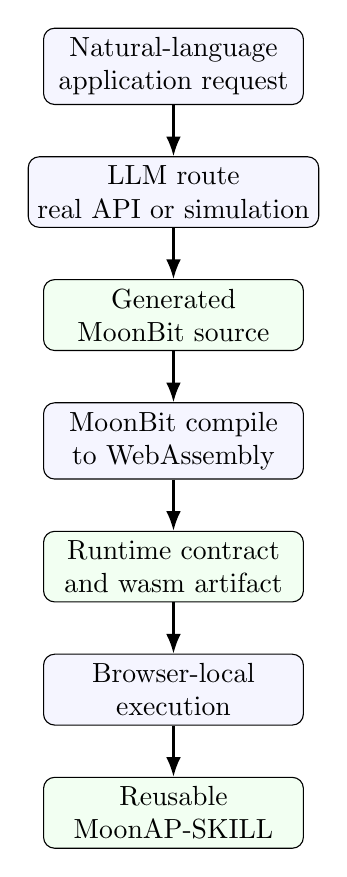
\begin{tikzpicture}[
  node distance=0.65cm,
  block/.style={draw, rounded corners, align=center, minimum width=3.3cm, minimum height=0.82cm, fill=blue!4},
  data/.style={draw, rounded corners, align=center, minimum width=3.3cm, minimum height=0.82cm, fill=green!5},
  arrow/.style={-{Latex[length=2.5mm]}, thick}
]
\node[block] (prompt) {Natural-language\\application request};
\node[block, below=of prompt] (router) {LLM route\\real API or simulation};
\node[data, below=of router] (source) {Generated\\MoonBit source};
\node[block, below=of source] (compile) {MoonBit compile\\to WebAssembly};
\node[data, below=of compile] (runtime) {Runtime contract\\and wasm artifact};
\node[block, below=of runtime] (browser) {Browser-local\\execution};
\node[data, below=of browser] (skill) {Reusable\\MoonAP-SKILL};
\draw[arrow] (prompt) -- (router);
\draw[arrow] (router) -- (source);
\draw[arrow] (source) -- (compile);
\draw[arrow] (compile) -- (runtime);
\draw[arrow] (runtime) -- (browser);
\draw[arrow] (browser) -- (skill);
\end{tikzpicture}
\caption{End-to-end \moonap{} workflow. The LLM participates in source generation, while browser-local execution and artifact reuse are controlled by the host system. Large user data files stay on the browser side of the workflow.}
\label{fig:pipeline}
\end{figure}

\begin{figure}[t]
\centering
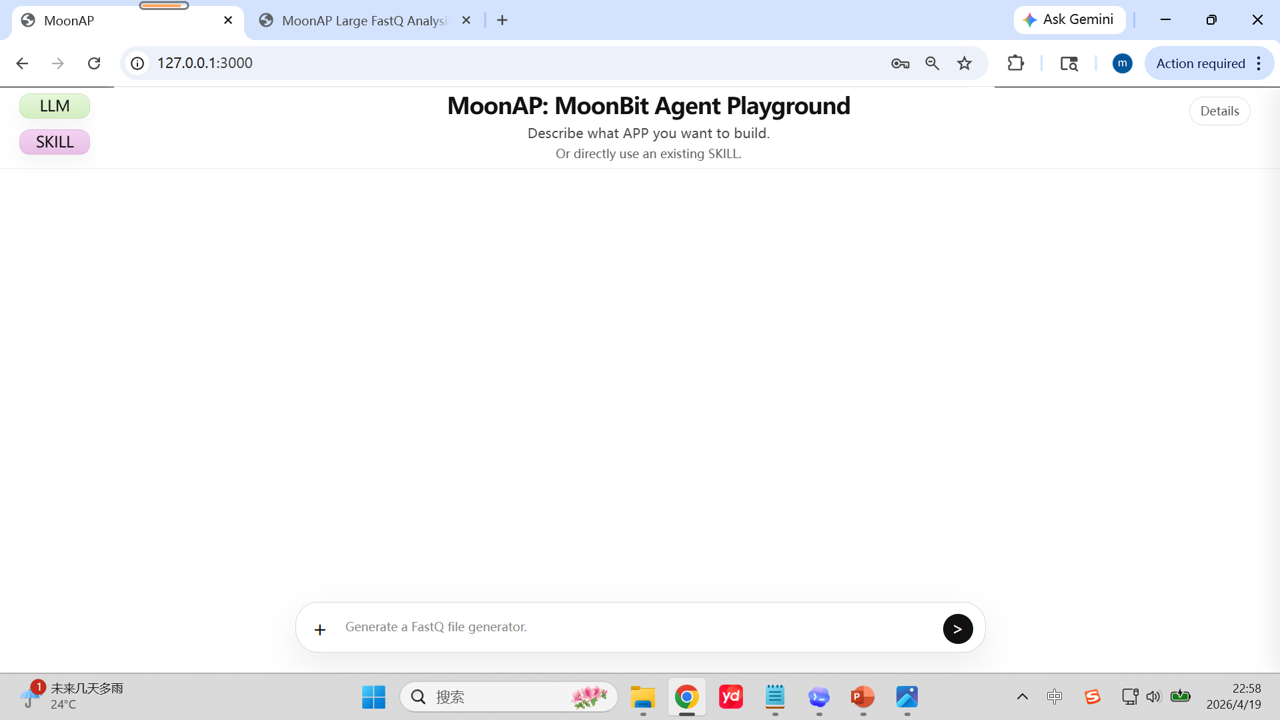
\includegraphics[width=0.94\linewidth]{figures/screenshot-main-ui.png}
\caption{\moonap{} browser UI. Users can enter a natural-language application request or switch to the \skill{} interface for reuse and installation.}
\label{fig:main-ui}
\end{figure}

\section{MoonAP-SKILL Architecture}

\moonap{}-\skill{}s are reusable application packages. A saved \skill{} contains a human-readable \texttt{SKILL.md}, generated MoonBit source, a compiled \wasm{} artifact, runtime metadata, and optional distribution files. The design goal is to make a generated application behave less like a transient chat response and more like a local tool that can be inspected, copied, installed, and rerun. The v0.1 design separates \skill{}s into three layers (Figure~\ref{fig:skill}).

\begin{figure}[t]
\centering
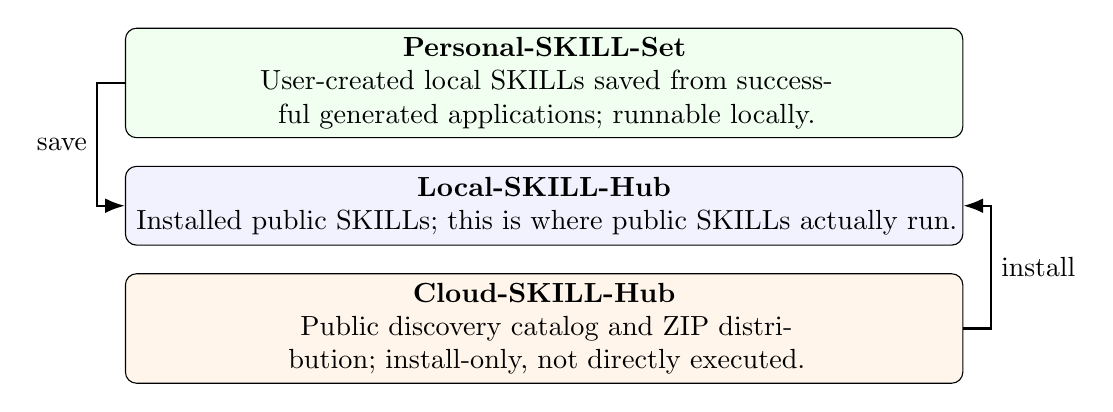
\begin{tikzpicture}[
  layer/.style={draw, rounded corners, text width=10.4cm, minimum height=1cm, align=center},
  arrow/.style={-{Latex[length=2.5mm]}, thick}
]
\node[layer, fill=green!6] (personal) {\textbf{Personal-SKILL-Set}\\User-created local \skill{}s saved from successful generated applications; runnable locally.};
\node[layer, fill=blue!5, below=0.35cm of personal] (local) {\textbf{Local-SKILL-Hub}\\Installed public \skill{}s; this is where public \skill{}s actually run.};
\node[layer, fill=orange!8, below=0.35cm of local] (cloud) {\textbf{Cloud-SKILL-Hub}\\Public discovery catalog and ZIP distribution; install-only, not directly executed.};
\draw[arrow] (cloud.east) -- ++(0.35,0) |- node[pos=0.25,right]{install} (local.east);
\draw[arrow] (personal.west) -- ++(-0.35,0) |- node[pos=0.25,left]{save} (local.west);
\end{tikzpicture}
\caption{Three-layer \moonap{}-\skill{} model. Cloud entries are used for discovery and installation; execution happens in Personal or Local stores.}
\label{fig:skill}
\end{figure}

This separation addresses three practical issues. First, it prevents cloud catalog entries from being treated as directly executable objects before they have been installed and inspected locally. Second, it gives the user a clear distinction between self-created artifacts and public artifacts obtained from a hub. Third, it separates discovery from execution: the cloud hub can advertise and distribute packages, while actual runs happen from local stores under the user's control. Figure~\ref{fig:skill-ui} shows the browser UI for selecting a Local-\skill{}-Hub directory, inspecting installed \skill{}s, refreshing the Cloud-\skill{}-Hub catalog, installing public \skill{}s, and running local \skill{}s.

\begin{figure}[t]
\centering
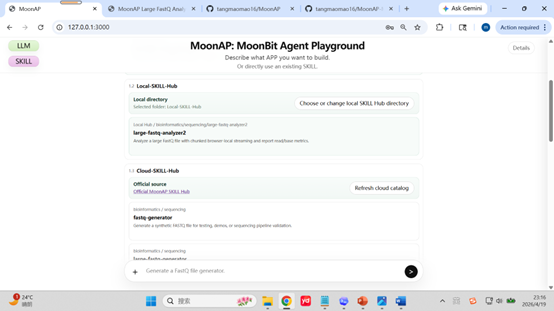
\includegraphics[width=0.94\linewidth]{figures/screenshot-local-cloud-skill.png}
\caption{\moonap{} Local-\skill{}-Hub and Cloud-\skill{}-Hub interface. Installed public \skill{}s run from the local hub, while cloud entries are used for discovery and installation.}
\label{fig:skill-ui}
\end{figure}

\section{Runtime Contracts}

One of the central lessons from v0.1 is that synthesized source code is not enough to produce a usable application. The host must know what input controls to render, whether an input file is required, how results should be displayed, and whether the output should be downloaded, shown as a report, or treated as an interactive view.

\moonap{} uses runtime contracts for this purpose. A runtime contract is a structured specification associated with a generated artifact. The contract is intentionally host-facing: it tells the browser what experience to provide around the compiled program. It can include:

\begin{itemize}[leftmargin=*]
  \item runtime mode, such as \texttt{form}, \texttt{file}, or \texttt{interactive};
  \item result mode, such as \texttt{text}, \texttt{report}, or \texttt{download};
  \item input fields with labels, types, default values, and validation hints;
  \item an I/O contract for file or large-file workflows;
  \item action labels and rerun labels for the UI;
  \item tool-specific metadata, such as CSV summary or FastQ analysis.
\end{itemize}

The runtime contract enables generic execution paths for many small tools. For example, the Celsius/Fahrenheit converter, minutes/seconds converter, BMI calculator, circle calculator, loan payment calculator, tip calculator, JSON formatter, and text analyzer can all be represented as form or text contracts. The CSV analyzer uses a file contract with a browser-local file picker and report output. Without this contract layer, each generated app would require bespoke front-end glue code or manual intervention before it could feel like a usable application.

The contract also makes \skill{} reuse possible. When a \skill{} is run again, \moonap{} does not need to ask the LLM to regenerate code. Instead, it reloads the saved runtime specification, renders the appropriate UI, and executes the local runtime path. This keeps the LLM call focused on creation and repair, not on every future use of the tool.

\section{Browser-Local Large-File Workflows}

\moonap{} v0.1 includes two large-file FastQ workflows: generation and analysis. These workflows are intentionally treated as high-value demonstrations of browser-local computation rather than as the only purpose of the platform. They also illustrate an important design point for LLM-generated applications: the LLM should help create the tool, but it should not need to ingest the user's raw data file.

\paragraph{Large FastQ generation.}
The generator uses a browser file-save picker and a streamed writer. The user chooses an output file, enters parameters such as target size, read length, random seed, and N-base rate, and the browser writes records locally. This design can produce large synthetic files, including 1GB-scale demonstrations, without constructing the whole file in server memory. The generated file contents are not sent to the LLM.

\paragraph{Large FastQ analysis.}
The analyzer uses a browser file-open picker and reads the selected file in chunks. It counts reads, lines, bases, base composition, malformed records, read lengths, and elapsed time. Because the raw bytes are processed through browser-local chunking, the workflow is suitable for large local files, including GB-scale demonstrations on commodity machines. File contents stay in the browser; the server receives only summary metrics and result metadata.

These workflows are important because they exercise a workload that ordinary chat-based code generation does not handle well. Sending a GB-scale data file to an LLM would be expensive, slow, and often impossible under token limits. In \moonap{}, the prompt and tool specification can be small, while the high-volume data path remains local.

Figure~\ref{fig:fastq-report} shows the browser-local FastQ report generated by the analyzer. The report is opened from a browser blob URL and presents summary metrics and base-composition results without uploading the original file contents.

\begin{figure}[t]
\centering
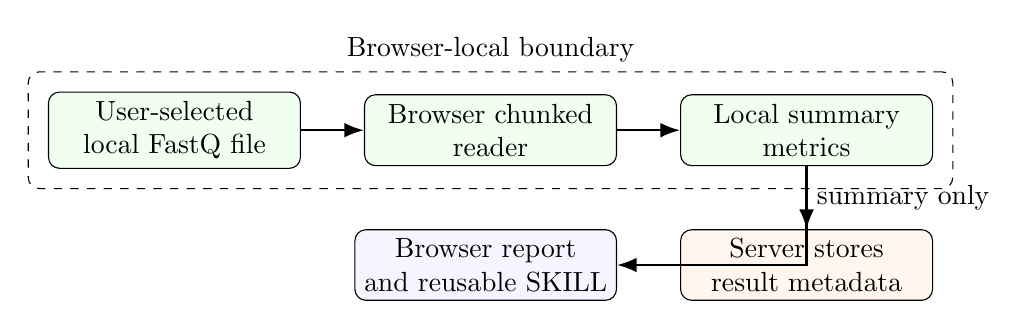
\begin{tikzpicture}[
  node distance=0.8cm,
  block/.style={draw, rounded corners, align=center, minimum width=3.2cm, minimum height=0.8cm, fill=blue!4},
  local/.style={draw, rounded corners, align=center, minimum width=3.2cm, minimum height=0.8cm, fill=green!6},
  server/.style={draw, rounded corners, align=center, minimum width=3.2cm, minimum height=0.8cm, fill=orange!7},
  arrow/.style={-{Latex[length=2.5mm]}, thick}
]
\node[local] (file) {User-selected\\local FastQ file};
\node[local, right=of file] (chunks) {Browser chunked\\reader};
\node[local, right=of chunks] (metrics) {Local summary\\metrics};
\node[server, below=of metrics] (record) {Server stores\\result metadata};
\node[block, left=of record] (report) {Browser report\\and reusable SKILL};
\draw[arrow] (file) -- (chunks);
\draw[arrow] (chunks) -- (metrics);
\draw[arrow] (metrics) -- node[right]{summary only} (record);
\draw[arrow] (metrics) |- (report);
\node[draw, dashed, rounded corners, fit=(file)(chunks)(metrics), inner sep=0.25cm, label=above:{Browser-local boundary}] {};
\end{tikzpicture}
\caption{Browser-local large-file analysis. File contents are processed in the browser; only summary metadata is recorded by the local server.}
\label{fig:largefile}
\end{figure}

\begin{figure}[t]
\centering
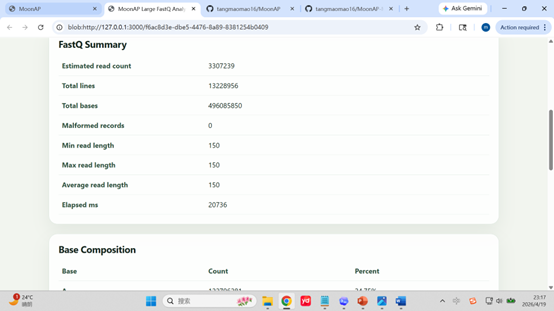
\includegraphics[width=0.94\linewidth]{figures/screenshot-fastq-summary-table.png}
\caption{FastQ analysis report with summary metrics and the beginning of the base-composition table. The counts are computed locally in the browser from the selected FastQ file.}
\label{fig:fastq-report}
\end{figure}

\section{Implementation}

The prototype is organized as a MoonBit project with a local server package and a browser application package. The server handles HTTP endpoints, LLM routing, runtime registration, artifact persistence, \skill{} export, and static file serving. The browser app implements the user interface, runtime cards, file pickers, generic runtime execution, large-file progress reporting, \skill{} installation, and \skill{} reuse.

The system currently targets a Windows-first release path. Native server builds use the MoonBit toolchain together with MSVC setup scripts. The browser side is compiled to JavaScript and committed as distribution bundles for fresh-clone startup fallback. The primary validated browser target is Chrome or Edge, because large-file workflows depend on the File System Access API~\cite{file-system-access}.

\subsection{LLM Routes}

\moonap{} separates real and simulated LLM routes. Real routes support multiple providers or OpenAI-compatible endpoints. The simulated route provides deterministic outputs for the v0.1 demo set. This distinction is important because real lightweight models often fail to produce valid MoonBit in the current ecosystem. The simulated route is not presented as an evaluation of model quality; it is a system-testing path that exercises the compile, runtime, and \skill{} reuse pipeline.

This choice keeps two claims separate. \moonap{} does not claim that every current LLM can reliably generate MoonBit. It claims that the surrounding platform can turn a successful or simulated generation into a compiled, runnable, reusable browser-local application. As MoonBit becomes more common in model training data and stronger providers improve, the same platform path can absorb better generation quality without changing the runtime architecture.

\subsection{Artifact Lifecycle}

The lifecycle of an artifact has four stages:

\begin{enumerate}[leftmargin=*]
  \item \textbf{Generation:} prompt and LLM output are captured.
  \item \textbf{Compilation:} MoonBit source is compiled into a \wasm{} artifact.
  \item \textbf{Runtime:} the browser executes a contract-driven runtime step and records a result.
  \item \textbf{Reuse:} the artifact is materialized as a \skill{} and later run from Personal-\skill{}-Set or Local-\skill{}-Hub.
\end{enumerate}

This lifecycle allows \moonap{} to treat a successful generated app as an asset rather than a transient response.

\section{Evaluation and Case Studies}

The v0.1 evaluation is qualitative and prototype-oriented. It asks whether the system can express, run, and reuse representative browser-local applications. Table~\ref{tab:demos} summarizes the current demonstration matrix.

The evaluation is organized around platform capability rather than model leaderboard accuracy. A demonstration category is considered successful when the system can produce or load the application, expose the correct runtime controls, run the browser-local workflow, present the result, and preserve the artifact for later reuse where applicable.

\begin{table}[t]
\centering
\small
\begin{tabular}{L{0.28\linewidth}L{0.42\linewidth}L{0.20\linewidth}}
\toprule
\textbf{Capability family} & \textbf{Examples} & \textbf{Runtime path}\\
\midrule
Computed form apps & Celsius/Fahrenheit, minutes/seconds, two-number sum, BMI, circle, loan, tip & Generic form contract\\
Text and JSON utilities & JSON formatter/validator, text analyzer & Generic text runtime\\
Browser-local file utility & CSV summary analyzer & Generic file/report runtime\\
Large-file generation & Large FastQ generator & Streamed browser writer\\
Large-file analysis & Large FastQ analyzer & Chunked browser reader/report\\
Reuse & Personal \skill{}, Local-\skill{}-Hub & Saved runtime spec\\
Sharing/install & Cloud-\skill{}-Hub & Catalog and ZIP install\\
\bottomrule
\end{tabular}
\caption{MoonAP v0.1 demonstration matrix.}
\label{tab:demos}
\end{table}

The small utility tasks exercise the generic contract path. They show that the browser can render task-specific controls without bespoke UI code for each generated app. The CSV analyzer extends this pattern to file input and report output. The FastQ generator and analyzer exercise specialized large-file runtime paths that rely on browser-local streaming and chunking. Together, the cases cover both ordinary utility apps and data-heavy local workflows.

The most important engineering result is the reuse path. A successful generated app can be saved as a \skill{}, reopened, and executed from a local store without another LLM call. This substantially changes the user experience: the LLM is used to create or repair an artifact, but the artifact can later behave like a normal local application.

\section{Lessons Learned}

\paragraph{Generated code needs a host contract.}
Without a runtime contract, the browser does not know which inputs to show or how to interpret results. Embedding or saving this contract makes generated apps reusable.

\paragraph{A deterministic path is necessary for system development.}
When the target language is young, real models may fail for reasons unrelated to the runtime system. The simulated route allowed v0.1 to test compilation, UI, file handling, and \skill{} reuse deterministically.

\paragraph{Reuse is as important as generation.}
Users should not need to pay the latency and uncertainty cost of an LLM call every time they run a useful generated app. The \skill{} format turns synthesis into a reusable software artifact. This also reduces repeated cloud LLM usage: the generative step is used for creation or repair, while repeated execution happens locally from the saved contract and compiled artifact.

\paragraph{Browser-local file boundaries must be explicit.}
For large files, privacy and performance depend on a clear boundary: file contents stay in the browser, while summaries and metadata can be recorded by the local server.

\paragraph{Client hardware is part of the execution platform.}
Browser-local \wasm{} execution lets \moonap{} use computation and storage resources already available on the user's device. This edge-side execution model is especially valuable for file utilities, where moving raw data to a cloud model would be slower, more expensive, and less private than processing it near the data.

\section{Limitations}

\moonap{} v0.1 has several limitations. First, real LLM generation of valid MoonBit is not yet reliable across lightweight or free models. Stronger models may perform better, but model capability and provider availability are external variables. Second, the current release path is best tested on Windows with Chrome or Edge; the File System Access API is not a universal browser baseline~\cite{mdn-file-system-access}. Third, the generic runtime contract is still small and does not yet cover arbitrary application UIs, complex stateful apps, or a universal \wasm{} host ABI. Fourth, the evaluation is a prototype case study rather than a large-scale benchmark. Finally, security hardening remains future work: generated code, saved artifacts, and hub-installed packages need stronger provenance and sandboxing mechanisms before broad deployment, a concern consistent with prior work on the security risks of generated code~\cite{pearce2022asleep}.

\section{Future Work}

Future versions of \moonap{} can extend the platform in several directions:

\begin{itemize}[leftmargin=*]
  \item a more formal runtime contract schema and validation layer;
  \item a stable host ABI for generated \wasm{} programs with file, stream, and UI callbacks;
  \item stronger automated repair loops for MoonBit compilation errors;
  \item cross-platform server support beyond the current Windows-first path;
  \item richer \skill{} provenance, signatures, versioning, and dependency management;
  \item quantitative evaluation over larger prompt suites and real model providers;
  \item improved UI generation for interactive applications and games.
\end{itemize}

\section{Conclusion}

\moonap{} v0.1 demonstrates an end-to-end MoonBit software synthesis workflow: natural-language task descriptions become MoonBit source, compiled \wasm{} artifacts, browser-local applications, and reusable \skill{} packages. The system highlights a practical lesson for LLM-based software synthesis: generation is only the first step. A usable platform also needs runtime contracts, local execution boundaries, artifact packaging, deterministic testing paths, and reuse mechanisms. By keeping raw data on the client, using browser-side computation for file workflows, and reusing saved \skill{}s without repeated generation, \moonap{} points toward a more privacy-preserving and cost-aware style of practical software synthesis. The v0.1 prototype is therefore not merely a FastQ demo or a code-generation wrapper; it is an application lifecycle platform for turning generated MoonBit programs into local tools. Although current lightweight LLMs do not yet generate MoonBit reliably, \moonap{} shows how a MoonBit-centered agent playground can make generated applications inspectable, runnable, reusable, and data-local in the browser.

\bibliographystyle{plain}
\bibliography{references}

\end{document}
